\documentclass[aspectratio=169,10pt]{beamer}
\usetheme{Madrid}
% ─── shared_preamble.tex  (input this from every document) ──────────────────

% Packages
\usepackage{amsmath,amssymb,bm}
\usepackage{booktabs,array,colortbl,multirow}
\usepackage{tikz}
\usetikzlibrary{arrows.meta,shapes,positioning,fit,backgrounds,calc,decorations.pathreplacing}
\usepackage{listings}
\usepackage{xcolor}
\usepackage{graphicx}
\usepackage{multicol}
\usepackage{tcolorbox}
\tcbuselibrary{skins,breakable}


% ── Palette  (Ocean deep: navy / teal / white / gold accent) ─────────────────
\definecolor{NavyD}  {RGB}{10,  38,  71}   % primary dark
\definecolor{TealM}  {RGB}{1,  102, 140}   % mid tone
\definecolor{TealL}  {RGB}{0,  168, 176}   % light accent
\definecolor{Gold}   {RGB}{255,185,  0}    % accent / highlight
\definecolor{OffW}   {RGB}{245,248,252}    % off-white body bg
\definecolor{SlateG} {RGB}{88, 110, 130}   % muted text
\definecolor{AlertR} {RGB}{192, 38,  38}   % warnings
\definecolor{GreenG} {RGB}{30, 120,  60}   % positive / correct

% ── Beamer colours ────────────────────────────────────────────────────────────
\setbeamercolor{palette primary}    {bg=NavyD, fg=white}
\setbeamercolor{palette secondary}  {bg=TealM, fg=white}
\setbeamercolor{palette tertiary}   {bg=TealL, fg=white}
\setbeamercolor{structure}          {fg=NavyD}
\setbeamercolor{section in toc}     {fg=NavyD}
\setbeamercolor{alerted text}       {fg=AlertR}
\setbeamercolor{block title}        {bg=NavyD, fg=white}
\setbeamercolor{block body}         {bg=OffW}
\setbeamercolor{block title alerted}{bg=AlertR, fg=white}
\setbeamercolor{block body alerted} {bg=red!5}
\setbeamercolor{block title example}{bg=GreenG, fg=white}
\setbeamercolor{block body example} {bg=green!4}
\setbeamercolor{frametitle}         {bg=NavyD, fg=white}
\setbeamercolor{background canvas}  {bg=OffW}
\setbeamerfont{frametitle}{size=\large,series=\bfseries}

% ── tcolorbox styles ──────────────────────────────────────────────────────────
\tcbset{
  mybox/.style={
    enhanced, boxrule=0pt, frame hidden,
    interior style={fill=NavyD!8},
    left=6pt, right=6pt, top=4pt, bottom=4pt,
    borderline west={3pt}{0pt}{TealM}
  },
  keybox/.style={
    enhanced, boxrule=1pt, colframe=Gold,
    interior style={fill=Gold!10},
    left=6pt, right=6pt, top=4pt, bottom=4pt
  },
  codebox/.style={
    enhanced, boxrule=0pt, frame hidden,
    interior style={fill=NavyD!5},
    left=4pt, right=4pt, top=2pt, bottom=2pt,
    borderline west={2pt}{0pt}{TealL}
  }
}

% ── Python listings ───────────────────────────────────────────────────────────
\lstdefinestyle{pycode}{
  language=Python,
  basicstyle=\ttfamily\scriptsize,
  keywordstyle=\color{TealM}\bfseries,
  stringstyle=\color{GreenG},
  commentstyle=\color{SlateG}\itshape,
  numberstyle=\tiny\color{SlateG},
  numbers=left, numbersep=5pt,
  breaklines=true,
  showstringspaces=false,
  frame=none,
  backgroundcolor=\color{NavyD!5},
  tabsize=4,
  morekeywords={import,from,as,True,False,None,print,len,range}
}

% ── Footer ────────────────────────────────────────────────────────────────────
\setbeamertemplate{navigation symbols}{}
\setbeamertemplate{footline}{%
  \leavevmode%
  \hbox{%
    \begin{beamercolorbox}[wd=.40\paperwidth,ht=2ex,dp=0.8ex,left,leftskip=4pt]{palette primary}%
      \usebeamerfont{author in head/foot}\small\insertshortauthor
    \end{beamercolorbox}%
    \begin{beamercolorbox}[wd=.35\paperwidth,ht=2ex,dp=0.8ex,center]{palette secondary}%
      \usebeamerfont{title in head/foot}\small\insertshorttitle
    \end{beamercolorbox}%
    \begin{beamercolorbox}[wd=.25\paperwidth,ht=2ex,dp=0.8ex,right,rightskip=4pt]{palette tertiary}%
      \small\insertframenumber\,/\,\inserttotalframenumber
    \end{beamercolorbox}}%
}

% ── Section title slide ───────────────────────────────────────────────────────
\AtBeginSection[]{
  \begin{frame}
    \begin{tikzpicture}[remember picture, overlay]
      \fill[NavyD] (current page.north west) rectangle (current page.south east);
      \fill[TealM!60] (current page.south west) rectangle +(\paperwidth,1.4cm);
      \node[white,font=\LARGE\bfseries, anchor=center]
        at (current page.center) {\insertsectionhead};
      \node[TealL,font=\normalsize, anchor=north]
        at ([yshift=-0.5cm]current page.center) {\secname};
    \end{tikzpicture}
  \end{frame}
}

% ── Convenience commands ──────────────────────────────────────────────────────
\newcommand{\bfemph}[1]{\textbf{\textcolor{TealM}{#1}}}
\newcommand{\gold}[1]{\textcolor{Gold}{\textbf{#1}}}
\newcommand{\imp}[1]{\textcolor{AlertR}{\textbf{#1}}}
\newcommand{\good}[1]{\textcolor{GreenG}{\textbf{#1}}}
\newcommand{\dataset}{\textit{FarmYield}}


\title[Day 1 — Linear Regression]{Machine Learning for Agricultural Science}
\subtitle{Day 1: Linear Regression --- From First Principles}
\author[ML Workshop]{ML Training Workshop}
\date{Day 1 of 4 \quad|\quad 2-Hour Theory Session}
\institute{Understanding How Inputs Drive Crop Yield}

\begin{document}

% ── Title ─────────────────────────────────────────────────────────────────────
\begin{frame}
  
\begin{tikzpicture}[remember picture,overlay]
    \fill[NavyD] (current page.north west) rectangle (current page.south east);
    \fill[TealM] (current page.south west) rectangle +(\paperwidth,2.2cm);
    \node[white,font=\huge\bfseries,anchor=south west]
      at ([xshift=0.7cm,yshift=2.4cm]current page.south west)
      {Machine Learning for Agricultural Science};
    \node[TealL,font=\Large,anchor=north west]
      at ([xshift=0.7cm,yshift=2.15cm]current page.south west)
      {Day 1 --- Linear Regression: From First Principles};
    \node[Gold,font=\normalsize,anchor=south east]
      at ([xshift=-0.7cm,yshift=0.15cm]current page.south east)
      {2-Hour Theory Session};
    \node[OffW,font=\small,anchor=north west]
      at ([xshift=0.7cm,yshift=-1.4cm]current page.north west)
      {No prior statistics experience required};
  \end{tikzpicture}
\end{frame}

% ── Roadmap ───────────────────────────────────────────────────────────────────
\begin{frame}{Four-Day Workshop Roadmap}
  \begin{center}
  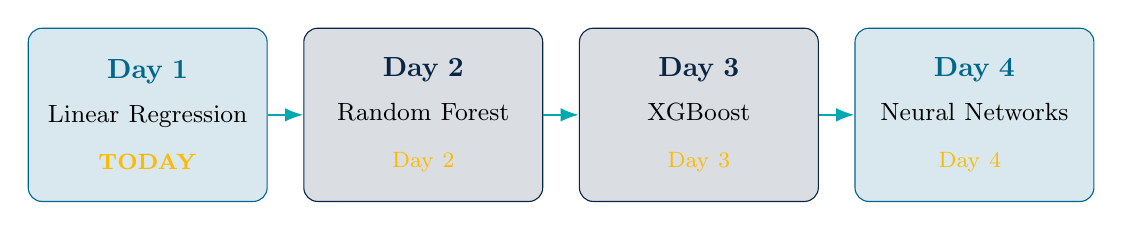
\begin{tikzpicture}
    \foreach \d/\t/\c/\s in {
      1/{Linear Regression}/TealM/{\textbf{TODAY}},
      2/{Random Forest}/NavyD/{Day 2},
      3/{XGBoost}/NavyD/{Day 3},
      4/{Neural Networks}/TealM/{Day 4}
    }{
      \node[draw=\c,fill=\c!15,rounded corners=5pt,
            minimum width=3.0cm,minimum height=2.2cm,
            text width=2.8cm,align=center,
            xshift={(\d-1)*3.5cm}] (d\d)
        {\textbf{\textcolor{\c}{Day \d}}\\[5pt]\small\t\\[5pt]\footnotesize\textcolor{Gold}{\s}};
    }
    \foreach \i in {1,2,3}{
      \pgfmathtruncatemacro{\j}{\i+1}
      \draw[-{Latex},TealL,thick] (d\i.east)--(d\j.west);
    }
  \end{tikzpicture}
  \end{center}
  \vspace{0.3cm}
  \begin{columns}
    \column{0.49\textwidth}
      \begin{tcolorbox}[mybox]
        \small\textbf{The Dataset: \dataset{}}\\[4pt]
        Crop yield from 1\,200 farms across 5 countries.
        You will apply each technique to the \textbf{same data all week}
        and compare results on the last day.
      \end{tcolorbox}
    \column{0.49\textwidth}
      \begin{tcolorbox}[keybox]
        \small\textbf{\textbf{*} Today's Goal}\\[4pt]
        Build and interpret a linear model that explains how rainfall,
        fertiliser and other factors drive wheat yield --- in plain language.
      \end{tcolorbox}
  \end{columns}
\end{frame}

\begin{frame}{Today's Session at a Glance}
  \tableofcontents[hideallsubsections]
\end{frame}

% ══════════════════════════════════════════════════════════════════════════════
\section{What is a Model and Why Do We Need One?}
% ══════════════════════════════════════════════════════════════════════════════

\begin{frame}{The Central Question}
  \begin{columns}
    \column{0.54\textwidth}
      \begin{tcolorbox}[keybox]
        \large\centering
        ``If I apply 10 more kg/ha of nitrogen fertiliser,\\
        how much extra yield should I expect?''
      \end{tcolorbox}
      \vspace{0.4cm}
      \textbf{Why is this hard to answer from data alone?}
      \begin{itemize}
        \item Every farm is different (soil, climate, variety)
        \item Many factors act at the same time
        \item We want a \emph{general} answer, not farm-by-farm
        \item We cannot run infinite controlled experiments
      \end{itemize}
      \vspace{0.3cm}
      \textbf{A model} is a mathematical summary of patterns in data that
      lets us predict and explain in a systematic way.
    \column{0.42\textwidth}
      \begin{center}
      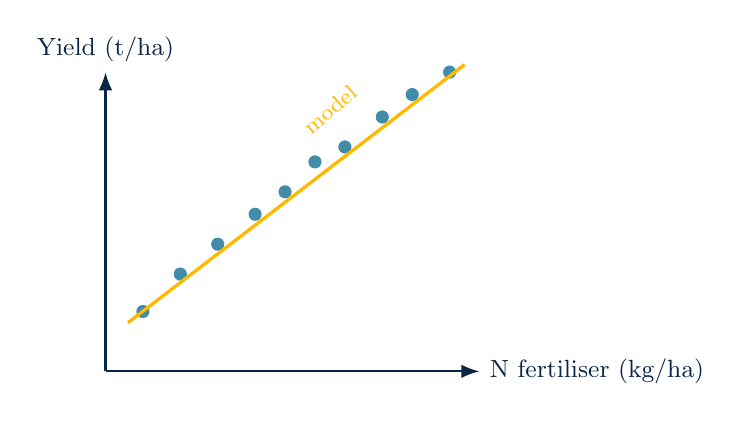
\begin{tikzpicture}[scale=0.95]
        \draw[-{Latex},NavyD,thick] (0,0)--(5,0)
          node[right,font=\small]{N fertiliser (kg/ha)};
        \draw[-{Latex},NavyD,thick] (0,0)--(0,4)
          node[above,font=\small]{Yield (t/ha)};
        \foreach \x/\y in {0.5/0.8,1.0/1.3,1.5/1.7,2.0/2.1,2.4/2.4,
                           2.8/2.8,3.2/3.0,3.7/3.4,4.1/3.7,4.6/4.0}{
          \fill[TealM,opacity=0.75] (\x,\y) circle (2.5pt);}
        \draw[Gold,very thick] (0.3,0.65)--(4.8,4.1);
        \node[Gold,font=\footnotesize,rotate=40] at (3.0,3.5) {model};
      \end{tikzpicture}
      \end{center}
      \small\centering Each dot = one farm.\\The line = what the model learned.
  \end{columns}
\end{frame}

\begin{frame}{Data Terminology Used All Week}
  \begin{columns}
    \column{0.52\textwidth}
      \begin{description}[\bfemph{Observation}]
        \item[\bfemph{Target} ($y$)]
          What we want to predict.
          \textit{Example: yield (t/ha)}
        \item[\bfemph{Features} ($x_1 \ldots x_p$)]
          Inputs used to predict.
          \textit{Example: rainfall, temperature, N fertiliser}
        \item[\bfemph{Observation}]
          One row of data = one farm.
        \item[\bfemph{Training data}]
          Farms the model learns from.
        \item[\bfemph{Test data}]
          New farms we predict --- never seen during training.
        \item[\bfemph{Model}]
          The learned relationship: $\hat{y} \approx f(x)$
      \end{description}
    \column{0.44\textwidth}
      \begin{tcolorbox}[mybox,title={\small\bfseries \dataset{} Feature List}]
        \footnotesize
        \begin{tabular}{ll}
          \texttt{rainfall\_mm}  & seasonal rainfall \\
          \texttt{temp\_mean\_c} & mean temperature \\
          \texttt{soil\_ph}      & soil acidity \\
          \texttt{N\_kg\_ha}     & nitrogen applied \\
          \texttt{P\_kg\_ha}     & phosphorus applied \\
          \texttt{elevation\_m}  & farm altitude \\
          \texttt{season\_days}  & growing season \\
          \texttt{irrigated}     & 0 = no, 1 = yes \\
          \texttt{crop\_variety} & A, B, or C \\
          \texttt{pest\_index}   & 0--10 \\
          \midrule
          \texttt{yield\_t\_ha}  & \textbf{TARGET} \\
        \end{tabular}
      \end{tcolorbox}
  \end{columns}
\end{frame}

% ══════════════════════════════════════════════════════════════════════════════
\section{Simple Linear Regression}
% ══════════════════════════════════════════════════════════════════════════════

\begin{frame}{The Simplest Possible Model: One Input}
  \begin{columns}
    \column{0.50\textwidth}
      Suppose we predict yield using only rainfall:
      \[
        \hat{y} = \beta_0 + \beta_1 \cdot x
      \]
      \begin{tcolorbox}[mybox]
        \footnotesize
        \begin{tabular}{lp{5cm}}
          $\hat{y}$ & predicted yield (t/ha) \\[2pt]
          $x$       & rainfall (mm) \\[2pt]
          $\beta_0$ & \textbf{intercept}: predicted yield when $x=0$ \\[2pt]
          $\beta_1$ & \textbf{slope}: extra yield per 1 mm of rain \\
        \end{tabular}
      \end{tcolorbox}
      \vspace{0.3cm}
      \textbf{Fitted result:}\quad $\hat{y} = 1.20 + 0.008 \cdot x$\\[6pt]
      \textbf{At 300 mm rain:}
      \[
        \hat{y} = 1.20 + 0.008 \times 300 = \mathbf{3.60}\text{ t/ha}
      \]
    \column{0.46\textwidth}
      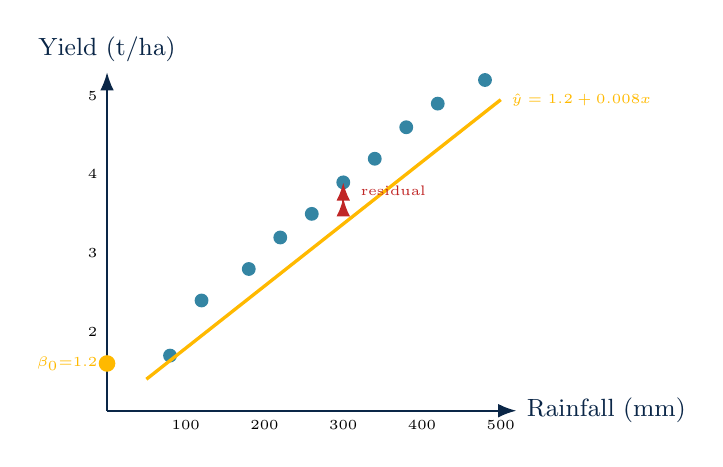
\begin{tikzpicture}[scale=1.0]
        \draw[-{Latex},NavyD,thick] (0,0)--(5.2,0)
          node[right,font=\small]{Rainfall (mm)};
        \draw[-{Latex},NavyD,thick] (0,0)--(0,4.3)
          node[above,font=\small]{Yield (t/ha)};
        \foreach \x/\l in {1/100,2/200,3/300,4/400,5/500}
          \node[below,font=\tiny] at (\x,0) {\l};
        \foreach \y/\l in {1/2,2/3,3/4,4/5}
          \node[left,font=\tiny] at (0,\y) {\l};
        \foreach \x/\y in {0.8/0.7,1.2/1.4,1.8/1.8,2.2/2.2,2.6/2.5,
                           3.0/2.9,3.4/3.2,3.8/3.6,4.2/3.9,4.8/4.2}{
          \fill[TealM,opacity=0.8] (\x,\y) circle (2.5pt);}
        \draw[Gold,very thick] (0.5,0.4)--(5.0,3.95)
          node[right,font=\tiny,Gold]{$\hat y=1.2+0.008x$};
        \draw[AlertR,thick,{Latex}-{Latex}] (3.0,2.7)--(3.0,2.9);
        \node[AlertR,right,font=\tiny] at (3.1,2.8) {residual};
        \fill[Gold] (0,0.6) circle (3pt);
        \node[Gold,left,font=\tiny] at (0,0.6) {$\beta_0$=1.2};
      \end{tikzpicture}
  \end{columns}
\end{frame}

\begin{frame}{The Slope and Intercept in Plain Language}
  \begin{columns}
    \column{0.48\textwidth}
      \begin{tcolorbox}[mybox,title={\bfseries Slope $\beta_1$ --- the key number}]
        \small $\beta_1 = +0.008$ means:\\[6pt]
        \textit{``Each extra mm of rainfall is associated with
        0.008 more t/ha of yield, on average.''}\\[8pt]
        \begin{tabular}{ll}
          $\beta_1 > 0$ & more $x \Rightarrow$ more yield \\
          $\beta_1 < 0$ & more $x \Rightarrow$ less yield \\
          $\beta_1 = 0$ & $x$ has no linear effect \\
        \end{tabular}
      \end{tcolorbox}
    \column{0.48\textwidth}
      \begin{tcolorbox}[mybox,title={\bfseries Intercept $\beta_0$ --- handle with care}]
        \small $\beta_0 = 1.20$ means:\\[6pt]
        \textit{``Predicted yield when rainfall = 0 mm.''}\\[8pt]
        Often has no practical meaning --- rainfall = 0 never occurs.\\[6pt]
        \imp{Do not over-interpret $\beta_0$} unless $x = 0$ is meaningful
        in your context.
      \end{tcolorbox}
  \end{columns}
  \vspace{0.4cm}
  \begin{tcolorbox}[keybox]
    \small\textbf{\textbf{*} The slope $\beta_1$ is what drives decisions.}
    It tells us how much yield responds to a unit change in the input ---
    this is what informs fertiliser rates, irrigation investment, etc.
  \end{tcolorbox}
\end{frame}

\begin{frame}{Residuals: Measuring How Wrong the Model Is}
  \begin{columns}
    \column{0.52\textwidth}
      No line fits every farm perfectly.
      The \textbf{residual} for farm $i$ is:
      \[
        e_i = y_i - \hat{y}_i \quad \text{(actual $-$ predicted)}
      \]
      \begin{center}
      \small
      \begin{tabular}{ccccc}
        \toprule
        Farm & Rain & Actual & Predicted & Residual \\
        \midrule
        1 & 200 & 2.8 & 2.8 & \textcolor{SlateG}{0.0} \\
        2 & 300 & 3.9 & 3.6 & \good{+0.3} \\
        3 & 300 & 3.2 & 3.6 & \imp{$-$0.4} \\
        4 & 400 & 4.1 & 4.4 & \imp{$-$0.3} \\
        5 & 500 & 5.3 & 5.2 & \good{+0.1} \\
        \bottomrule
      \end{tabular}
      \end{center}
      \vspace{0.2cm}
      \small
      Positive residual = model \textit{under}-predicted\\
      Negative residual = model \textit{over}-predicted
    \column{0.44\textwidth}
      \begin{tcolorbox}[mybox]
        \small\textbf{Why residuals matter:}\\[4pt]
        \begin{itemize}
          \item Show \textit{where} the model struggles
          \item Large residuals = poor fit for those farms
          \item Systematic patterns = model is missing something important
          \item Used to measure overall quality
          \item Used to check model assumptions
        \end{itemize}
      \end{tcolorbox}
      \vspace{0.2cm}
      \begin{tcolorbox}[keybox]
        \small A perfect model would have all residuals = 0.
        In practice, some residual error is always present
        due to factors we cannot measure.
      \end{tcolorbox}
  \end{columns}
\end{frame}

\begin{frame}{How the Best Line is Found: Least Squares}
  \begin{columns}
    \column{0.52\textwidth}
      We want to find the $\beta_0$ and $\beta_1$ that minimise the total error.\\[8pt]
      \textbf{Ordinary Least Squares (OLS)} minimises the
      \textbf{Sum of Squared Residuals}:
      \[
        \text{SSR} = \sum_{i=1}^{n}(y_i - \hat{y}_i)^2
      \]
      \begin{tcolorbox}[mybox]
        \small\textbf{Why square?}
        \begin{itemize}
          \item Makes positive and negative errors both count
          \item Penalises large errors more than small ones
          \item Has a clean analytical solution (no trial and error)
        \end{itemize}
      \end{tcolorbox}
      \vspace{0.2cm}
      \small\textbf{The solution is unique} --- there is exactly one best line
      for any dataset.
    \column{0.44\textwidth}
      \begin{center}
      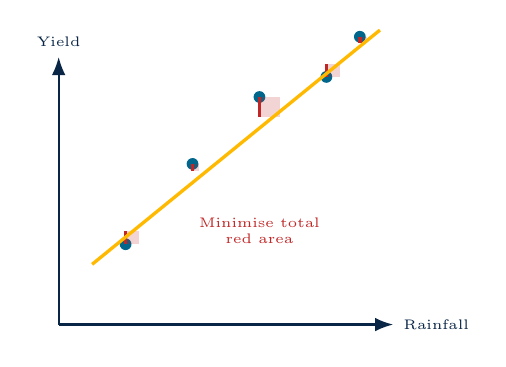
\begin{tikzpicture}[scale=0.85]
        \draw[-{Latex},NavyD,thick] (0,0)--(5,0) node[right,font=\tiny]{Rainfall};
        \draw[-{Latex},NavyD,thick] (0,0)--(0,4) node[above,font=\tiny]{Yield};
        \foreach \x/\y/\yh in {1.0/1.2/1.4, 2.0/2.4/2.3, 3.0/3.4/3.1,
                                4.0/3.7/3.9, 4.5/4.3/4.2}{
          \fill[TealM] (\x,\y) circle (2.5pt);
          \draw[AlertR,very thick] (\x,\y)--(\x,\yh);
          \pgfmathsetmacro{\wd}{abs(\y-\yh)}
          \fill[AlertR,opacity=0.2]
            (\x,\y) rectangle (\x+\wd,\yh);
        }
        \draw[Gold,very thick] (0.5,0.9)--(4.8,4.4);
        \node[AlertR,font=\tiny,align=center] at (3.0,1.4)
          {Minimise total\\red area};
      \end{tikzpicture}
      \end{center}
      \small\centering OLS finds the line that minimises the total squared residuals.
  \end{columns}
\end{frame}

% ══════════════════════════════════════════════════════════════════════════════
\section{Multiple Linear Regression}
% ══════════════════════════════════════════════════════════════════════════════

\begin{frame}{Using All Features Together}
  \begin{columns}
    \column{0.52\textwidth}
      Extend to $p$ features:
      \[
        \hat{y} = \beta_0 + \beta_1 x_1 + \beta_2 x_2 + \cdots + \beta_p x_p
      \]
      \vspace{0.1cm}
      \textbf{For \dataset{}:}
      \begin{align*}
        \hat{y} =\;& \beta_0 \\
        +\;&\beta_1 \cdot \text{rainfall} \\
        +\;&\beta_2 \cdot \text{temperature} \\
        +\;&\beta_3 \cdot \text{N\_fertiliser} \\
        +\;&\beta_4 \cdot \text{soil\_pH} + \cdots
      \end{align*}
    \column{0.44\textwidth}
      \begin{tcolorbox}[keybox,title={\bfseries Critical Concept}]
        \small Each $\beta_j$ is the effect of $x_j$\\
        \textbf{holding all other features constant}.\\[8pt]
        This is what ``controlling for other factors'' means.\\[8pt]
        \textbf{Example:} $\beta_3 = 0.048$ for N fertiliser means:\\
        \textit{Each extra kg/ha of N increases yield by 0.048 t/ha,
        for farms with the \textbf{same} rainfall, temperature and soil pH.}
      \end{tcolorbox}
  \end{columns}
\end{frame}

\begin{frame}{Reading the Regression Output Table}
  \textbf{Fitted model from \dataset{} --- example output:}
  \vspace{0.2cm}
  \begin{center}
  \small
  \begin{tabular}{lrrrl}
    \toprule
    \textbf{Feature} & \textbf{Coeff.\ $\hat\beta$} & \textbf{Std.\ Err.} & \textbf{$p$-value} & \textbf{Meaning} \\
    \midrule
    Intercept         & $-$1.83 & 0.42 & 0.001 & baseline (context-free) \\
    Rainfall (mm)     & $+$0.009 & 0.001 & $<$0.001 & +0.009 t/ha per mm \\
    Temperature (°C)  & $-$0.11  & 0.03  & 0.001 & $-$0.11 t/ha per °C \\
    N fertiliser      & $+$0.048 & 0.005 & $<$0.001 & +0.048 t/ha per kg/ha \\
    Soil pH           & $+$0.62  & 0.14  & 0.008 & +0.62 t/ha per pH unit \\
    Elevation (m)     & $-$0.002 & 0.001 & 0.12 & \textcolor{SlateG}{not significant} \\
    Season length     & $+$0.012 & 0.003 & 0.003 & longer season helps \\
    Irrigated (0/1)   & $+$0.74  & 0.11  & $<$0.001 & +0.74 t/ha if irrigated \\
    Pest index        & $-$0.18  & 0.04  & $<$0.001 & higher pests = less yield \\
    \bottomrule
  \end{tabular}
  \end{center}
  \begin{tcolorbox}[mybox]
    \small \textbf{How to read this:} (1) sign tells direction; (2) magnitude tells size; (3) $p<0.05$ means the effect is statistically detectable; (4) std.\ error measures precision.
  \end{tcolorbox}
\end{frame}

\begin{frame}{Categorical Variables: Dummy Coding}
  \begin{columns}
    \column{0.52\textwidth}
      \texttt{crop\_variety} takes values A, B, C --- not numbers.\\
      We convert using \textbf{dummy (indicator) variables}:
      \vspace{0.3cm}
      \begin{center}
      \small
      \begin{tabular}{lccc}
        \toprule
        Variety & $D_B$ & $D_C$ & Role \\
        \midrule
        A & 0 & 0 & \textit{reference} \\
        B & 1 & 0 & compared to A \\
        C & 0 & 1 & compared to A \\
        \bottomrule
      \end{tabular}
      \end{center}
      \vspace{0.3cm}
      \[
        \hat{y} = \cdots + \beta_B D_B + \beta_C D_C
      \]
      If $\beta_B = +0.32$: Variety B yields 0.32\,t/ha more than Variety A,
      all else equal.
    \column{0.44\textwidth}
      \begin{tcolorbox}[mybox]
        \small\textbf{Why not code A=1, B=2, C=3?}\\[4pt]
        That implies C is ``3 times'' A, which is meaningless for variety names.
        Dummy coding treats categories as distinct groups.
      \end{tcolorbox}
      \vspace{0.3cm}
      \begin{tcolorbox}[keybox]
        \small\textbf{Rule:} $k$ categories need $k-1$ dummies.\\[4pt]
        The omitted category is the \textbf{reference}. All coefficients
        are interpreted \textit{relative to it}.\\[4pt]
        \texttt{pd.get\_dummies(df, drop\_first=True)} does this automatically.
      \end{tcolorbox}
  \end{columns}
\end{frame}

% ══════════════════════════════════════════════════════════════════════════════
\section{Evaluating the Model}
% ══════════════════════════════════════════════════════════════════════════════

\begin{frame}{R-Squared: Proportion of Variation Explained}
  \begin{columns}
    \column{0.52\textwidth}
      \[
        R^2 = 1 - \frac{\text{SSR}}{\text{SST}}
        = 1 - \frac{\sum(y_i-\hat{y}_i)^2}{\sum(y_i-\bar{y})^2}
      \]
      \begin{tcolorbox}[mybox]
        \small SSR = variation left unexplained by model\\
        SST = total variation in yield (before model)
      \end{tcolorbox}
      \vspace{0.3cm}
      \begin{center}
      \small
      \begin{tabular}{cl}
        \toprule
        $R^2$ & Interpretation \\
        \midrule
        0.0 & Model explains nothing \\
        0.5 & Explains 50\% of variation \\
        0.78 & \dataset{} result --- good \\
        1.0 & Perfect (impossible in practice) \\
        \bottomrule
      \end{tabular}
      \end{center}
    \column{0.44\textwidth}
      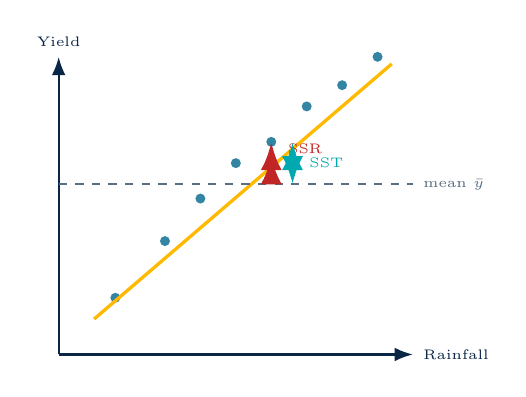
\begin{tikzpicture}[scale=0.9]
        \draw[-{Latex},NavyD,thick] (0,0)--(5,0) node[right,font=\tiny]{Rainfall};
        \draw[-{Latex},NavyD,thick] (0,0)--(0,4.2) node[above,font=\tiny]{Yield};
        \foreach \x/\y in {0.8/0.8,1.5/1.6,2.0/2.2,2.5/2.7,
                           3.0/3.0,3.5/3.5,4.0/3.8,4.5/4.2}{
          \fill[TealM,opacity=0.8] (\x,\y) circle (2pt);}
        \draw[Gold,very thick] (0.5,0.5)--(4.7,4.1);
        \draw[SlateG,dashed,thick] (0,2.4)--(5,2.4)
          node[right,font=\tiny]{mean $\bar y$};
        \draw[AlertR,ultra thick,{Latex}-{Latex}] (3.0,2.8)--(3.0,3.0);
        \node[AlertR,right,font=\tiny] at (3.1,2.9) {SSR};
        \draw[TealL,ultra thick,{Latex}-{Latex}] (3.3,2.4)--(3.3,3.0);
        \node[TealL,right,font=\tiny] at (3.4,2.7) {SST};
      \end{tikzpicture}
      \vspace{0.1cm}
      \small\centering $R^2 = 1 - \text{SSR}/\text{SST}$
  \end{columns}
\end{frame}

\begin{frame}{RMSE and MAE: Error in Real Units}
  \begin{columns}
    \column{0.48\textwidth}
      \begin{tcolorbox}[mybox,title={\bfseries Root Mean Squared Error}]
        \[
          \text{RMSE} = \sqrt{\frac{1}{n}\sum(y_i-\hat{y}_i)^2}
        \]
        \small\begin{itemize}
          \item In same units as yield (t/ha)
          \item Penalises large errors more
          \item \dataset{}: RMSE = 0.38 t/ha
        \end{itemize}
      \end{tcolorbox}
    \column{0.48\textwidth}
      \begin{tcolorbox}[mybox,title={\bfseries Mean Absolute Error}]
        \[
          \text{MAE} = \frac{1}{n}\sum|y_i-\hat{y}_i|
        \]
        \small\begin{itemize}
          \item In same units as yield (t/ha)
          \item All errors weighted equally
          \item Less sensitive to outliers
          \item \dataset{}: MAE = 0.30 t/ha
        \end{itemize}
      \end{tcolorbox}
  \end{columns}
  \vspace{0.4cm}
  \begin{tcolorbox}[keybox]
    \small\textbf{Both must be evaluated on test data --- farms the model has never seen.}
    Report both: RMSE for model comparison; MAE for communicating to stakeholders
    (``predictions are typically within 0.30 t/ha'').
  \end{tcolorbox}
\end{frame}

\begin{frame}{Train/Test Split and Cross-Validation}
  \begin{columns}
    \column{0.50\textwidth}
      \textbf{Train/Test Split:}
      \begin{center}
      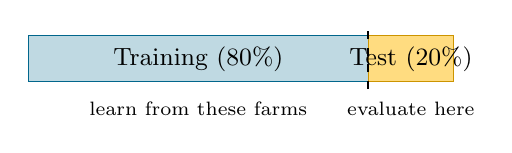
\begin{tikzpicture}[scale=0.9]
        \draw[fill=TealM!25,draw=TealM] (0,0) rectangle (4.8,0.65);
        \draw[fill=Gold!50,draw=Gold!80!black] (4.8,0) rectangle (6.0,0.65);
        \node[font=\small] at (2.4,0.32) {Training (80\%)};
        \node[font=\small] at (5.4,0.32) {Test (20\%)};
        \draw[dashed,thick] (4.8,-0.1)--(4.8,0.75);
        \node[font=\scriptsize,below] at (2.4,-0.15) {learn from these farms};
        \node[font=\scriptsize,below] at (5.4,-0.15) {evaluate here};
      \end{tikzpicture}
      \end{center}
      \vspace{0.5cm}
      \textbf{5-Fold Cross-Validation:}
      \begin{center}
      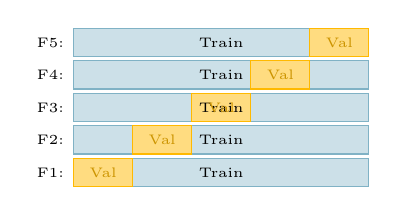
\begin{tikzpicture}[scale=0.75]
        \foreach \r/\y in {0/0,1/0.55,2/1.1,3/1.65,4/2.2}{
          \draw[fill=TealM!20,draw=TealM!50] (0,\y) rectangle (5.0,\y+0.48);
          \draw[fill=Gold!50,draw=Gold] (\r,\y) rectangle (\r+1,\y+0.48);
          \node[font=\tiny] at (2.5,\y+0.24) {Train};
          \node[font=\tiny,Gold!80!black] at (\r+0.5,\y+0.24) {Val};
          \pgfmathtruncatemacro{\fn}{\r+1}
          \node[font=\tiny,left] at (0,\y+0.24) {F\fn:};
        }
      \end{tikzpicture}
      \end{center}
    \column{0.46\textwidth}
      \begin{tcolorbox}[mybox]
        \small\textbf{When to use cross-validation:}\\[4pt]
        Preferred when the dataset is small (fewer than a few hundred observations).
        Every farm is used for both training and validation.\\[6pt]
        Report mean $\pm$ std across folds:\\
        $R^2 = 0.76 \pm 0.03$
      \end{tcolorbox}
      \vspace{0.3cm}
      \begin{tcolorbox}[keybox]
        \small\imp{Never report only training error.}\\
        A model that memorises training data looks perfect in-sample
        but will fail on new farms.
      \end{tcolorbox}
  \end{columns}
\end{frame}

\begin{frame}{Statistical Significance and $p$-values}
  \begin{columns}
    \column{0.52\textwidth}
      For each coefficient: \textit{Is this effect real, or could it
      have appeared by chance?}
      \begin{tcolorbox}[mybox]
        \small The \textbf{$p$-value} is the probability of seeing a
        coefficient at least this large if the true effect were zero.\\[6pt]
        \begin{tabular}{ll}
          $p < 0.05$ & \good{evidence of real effect} \\
          $p > 0.05$ & \textcolor{SlateG}{inconclusive} \\
        \end{tabular}
      \end{tcolorbox}
    \column{0.44\textwidth}
      \begin{tcolorbox}[keybox,title={\bfseries Important Caveats}]
        \small
        \begin{itemize}
          \item Significance $\neq$ importance\\
                A significant but tiny $\beta$ may have no practical impact
          \item Large datasets make almost everything significant
          \item Small datasets may miss real effects
          \item Always report both coefficient \textit{and} $p$-value
          \item 0.05 is a convention, not a physical law
        \end{itemize}
      \end{tcolorbox}
  \end{columns}
\end{frame}

% ══════════════════════════════════════════════════════════════════════════════
\section{Assumptions and Diagnostics}
% ══════════════════════════════════════════════════════════════════════════════

\begin{frame}{The Four Assumptions of Linear Regression (LINE)}
  \begin{columns}
    \column{0.50\textwidth}
      \begin{enumerate}
        \setlength\itemsep{0.35cm}
        \item[\textbf{L}] \textbf{Linearity}\\
              \small The true relationship is linear.
              A curved relationship will bias the estimates.
        \item[\textbf{I}] \textbf{Independence}\\
              \small Each farm's error is independent of others.
              Violated with repeated measurements on same farm.
        \item[\textbf{N}] \textbf{Normality of residuals}\\
              \small Residuals follow a normal distribution.
              Needed for valid $p$-values (less critical with $n>100$).
        \item[\textbf{E}] \textbf{Equal variance}\\
              \small Residuals have constant spread across all fitted values.
              Violated when high-yield farms are far more variable.
      \end{enumerate}
    \column{0.46\textwidth}
      \begin{tcolorbox}[keybox]
        \textbf{Memory aid: LINE}\\[4pt]
        \small \textbf{L}inearity\\
        \textbf{I}ndependence\\
        \textbf{N}ormality\\
        \textbf{E}qual variance
      \end{tcolorbox}
      \vspace{0.3cm}
      \begin{tcolorbox}[mybox]
        \small\textbf{Do not panic if mildly violated.}
        Linear regression is robust to mild violations, especially
        with samples of 100+.\\[4pt]
        Serious violations: use transformations,
        or switch to a non-linear model later this week.
      \end{tcolorbox}
  \end{columns}
\end{frame}

\begin{frame}{Diagnostic Plots: Check Assumptions Visually}
  \begin{columns}
    \column{0.50\textwidth}
      \textbf{Residuals vs Fitted} (check linearity \& equal variance)\\
      \small Random scatter = assumptions met
      \vspace{0.2cm}
      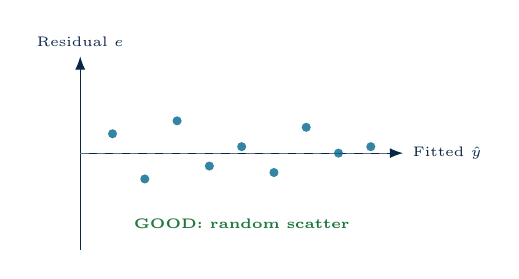
\begin{tikzpicture}[scale=0.82]
        \draw[-{Latex},NavyD] (0,1.5)--(5,1.5)
          node[right,font=\tiny]{Fitted $\hat y$};
        \draw[-{Latex},NavyD] (0,0)--(0,3) node[above,font=\tiny]{Residual $e$};
        \draw[dashed,SlateG] (0,1.5)--(4.8,1.5);
        \foreach \x/\y in {0.5/1.8,1/1.1,1.5/2.0,2/1.3,2.5/1.6,
                           3/1.2,3.5/1.9,4/1.5,4.5/1.6}{
          \fill[TealM,opacity=0.8] (\x,\y) circle (2pt);}
        \node[GreenG,font=\tiny] at (2.5,0.4) {\good{GOOD: random scatter}};
      \end{tikzpicture}

      \vspace{0.3cm}
      \textbf{Normal Q-Q plot} (check normality)\\
      \small Points falling on the diagonal = normal residuals
    \column{0.46\textwidth}
      \textbf{Scale-Location} (check equal variance)\\
      \small Flat line = variance is constant
      \vspace{0.2cm}
      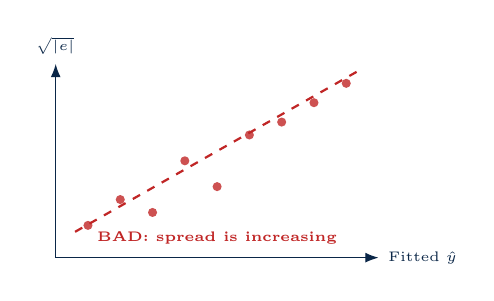
\begin{tikzpicture}[scale=0.82]
        \draw[-{Latex},NavyD] (0,0)--(5,0)
          node[right,font=\tiny]{Fitted $\hat y$};
        \draw[-{Latex},NavyD] (0,0)--(0,3) node[above,font=\tiny]{$\sqrt{|e|}$};
        \foreach \x/\y in {0.5/0.5,1/0.9,1.5/0.7,2/1.5,2.5/1.1,
                           3/1.9,3.5/2.1,4/2.4,4.5/2.7}{
          \fill[AlertR,opacity=0.8] (\x,\y) circle (2pt);}
        \draw[AlertR,dashed,thick] (0.3,0.4)--(4.7,2.9);
        \node[AlertR,font=\tiny] at (2.5,0.3) {\imp{BAD: spread is increasing}};
      \end{tikzpicture}
      \vspace{0.1cm}
      \begin{tcolorbox}[mybox]
        \small\textbf{In Python:}\\
        \texttt{statsmodels} produces all diagnostic plots via:\\
        \texttt{sm.graphics.plot\_regress\_exog()}\\
        You will generate these in today's practical.
      \end{tcolorbox}
  \end{columns}
\end{frame}

% ══════════════════════════════════════════════════════════════════════════════
\section{Python Implementation}
% ══════════════════════════════════════════════════════════════════════════════

\begin{frame}[fragile]{Linear Regression in Python}
  \begin{columns}
    \column{0.50\textwidth}
      \begin{tcolorbox}[codebox,title={\small\bfseries scikit-learn: for prediction}]
        \begin{lstlisting}[style=pycode]
import pandas as pd, numpy as np
from sklearn.linear_model import LinearRegression
from sklearn.model_selection import train_test_split
from sklearn.metrics import r2_score, mean_squared_error

df = pd.read_csv('farmyield.csv')
# Dummy-code crop_variety
df = pd.get_dummies(df,
     columns=['crop_variety'], drop_first=True)

X = df.drop(columns=['yield_t_ha'])
y = df['yield_t_ha']

X_train, X_test, y_train, y_test = \
    train_test_split(X, y, test_size=0.2,
                     random_state=42)
lr = LinearRegression()
lr.fit(X_train, y_train)
y_pred = lr.predict(X_test)

rmse = np.sqrt(mean_squared_error(y_test, y_pred))
r2   = r2_score(y_test, y_pred)
print(f"RMSE={rmse:.3f}  R2={r2:.3f}")
        \end{lstlisting}
      \end{tcolorbox}
    \column{0.46\textwidth}
      \begin{tcolorbox}[codebox,title={\small\bfseries statsmodels: for inference}]
        \begin{lstlisting}[style=pycode]
import statsmodels.api as sm

# Add constant for intercept
X_sm = sm.add_constant(X_train)
model = sm.OLS(y_train, X_sm).fit()

# Full summary: coefficients,
# std errors, t-stats, p-values,
# confidence intervals, R2
print(model.summary())

# Coefficient table only
print(model.params)      # beta values
print(model.pvalues)     # p-values
print(model.conf_int())  # 95% CI

# Diagnostic plots
import matplotlib.pyplot as plt
fig = sm.graphics.plot_regress_exog(
    model, 'N_kg_ha')
plt.show()
        \end{lstlisting}
      \end{tcolorbox}
  \end{columns}
\end{frame}

% ══════════════════════════════════════════════════════════════════════════════
\section{Limitations and the Road Ahead}
% ══════════════════════════════════════════════════════════════════════════════

\begin{frame}{When Linear Regression is Not Enough}
  \begin{columns}
    \column{0.50\textwidth}
      Linear regression assumes a straight-line relationship.
      Many agricultural effects are curved:
      \vspace{0.2cm}
      \begin{itemize}
        \setlength\itemsep{0.25cm}
        \item \textbf{Nitrogen response:} yield rises fast, then levels off
        \item \textbf{Temperature:} optimal range, drops at extremes
        \item \textbf{Interactions:} rain matters more in sandy soil
        \item \textbf{Thresholds:} zero yield below minimum water
      \end{itemize}
      \vspace{0.3cm}
      \begin{tcolorbox}[keybox]
        \small This is why we study more flexible models this week.
        But linear regression remains the baseline --- always build it first
        before trying complex models.
      \end{tcolorbox}
    \column{0.46\textwidth}
      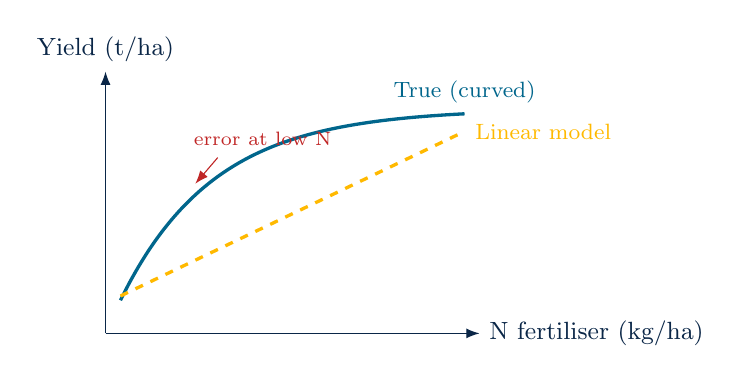
\begin{tikzpicture}[scale=0.95]
        \draw[-{Latex},NavyD] (0,0)--(5,0)
          node[right,font=\small]{N fertiliser (kg/ha)};
        \draw[-{Latex},NavyD] (0,0)--(0,3.5)
          node[above,font=\small]{Yield (t/ha)};
        \draw[TealM,very thick,domain=0.2:4.8,smooth,samples=40]
          plot(\x,{3*(1-exp(-0.8*\x))})
          node[above,font=\footnotesize]{True (curved)};
        \draw[Gold,dashed,very thick] (0.2,0.5)--(4.8,2.7)
          node[right,font=\footnotesize]{Linear model};
        \draw[-{Latex},AlertR] (1.5,2.35)--(1.2,2.0);
        \node[AlertR,font=\scriptsize,align=center] at (2.1,2.6)
          {error at low N};
      \end{tikzpicture}
  \end{columns}
\end{frame}

\begin{frame}{Day 1 Summary}
  \begin{columns}
    \column{0.50\textwidth}
      \textbf{\textcolor{TealM}{What we covered:}}
      \begin{itemize}
        \setlength\itemsep{0.2cm}
        \item Why we build models
        \item $\hat{y} = \beta_0 + \beta_1 x$ and how to read it
        \item Residuals = actual $-$ predicted
        \item OLS: minimise sum of squared residuals
        \item Multiple regression: many features simultaneously
        \item Each $\beta$ = effect holding others constant
        \item Dummy coding for categories
        \item $R^2$, RMSE, MAE evaluation metrics
        \item Train/test split and cross-validation
        \item $p$-values and statistical significance
        \item LINE assumptions and diagnostic plots
        \item Python: scikit-learn + statsmodels
      \end{itemize}
    \column{0.46\textwidth}
      \begin{tcolorbox}[keybox,title={\bfseries\textbf{*} The Big Idea}]
        \small Linear regression is the \textbf{foundation} of every model
        in this course.\\[6pt]
        Every advanced method (Random Forest, XGBoost, Neural Networks)
        is solving the same problem --- predict $y$ from $x$ --- but
        without the linearity constraint.\\[6pt]
        When you understand linear regression, the rest of the course
        becomes much easier.
      \end{tcolorbox}
      \vspace{0.3cm}
      \begin{center}
        \large\textbf{Practical Session Follows}\\[4pt]
        \small See \textit{practical\_day1.pdf}
      \end{center}
  \end{columns}
\end{frame}

\end{document}
